%%%%%%%%%%%%%%%%%%%%%%%%%%%%%%%%%%%%%%%%%%%%%%%
%%% Template for lab reports used at STIMA
%%%%%%%%%%%%%%%%%%%%%%%%%%%%%%%%%%%%%%%%%%%%%%%

%%%%%%%%%%%%%%%%%%%%%%%%%%%%%% Sets the document class for the document
% Openany is added to remove the book style of starting every new chapter on an odd page (not needed for reports)
\documentclass[10pt,english, openany]{book}

%%%%%%%%%%%%%%%%%%%%%%%%%%%%%% Loading packages that alter the style
\usepackage[]{graphicx}
% \documentclass[11pt, a4paper]{article}
\usepackage{graphicx}
\usepackage{amsmath}
\usepackage{listings}
\usepackage[]{color}
\usepackage{alltt}
\usepackage{amsmath, amssymb}
\usepackage[T1]{fontenc}
\usepackage[utf8]{inputenc}
\usepackage{lipsum}
\setcounter{secnumdepth}{3}
\setcounter{tocdepth}{3}
\setlength{\parskip}{\smallskipamount}
\setlength{\parindent}{0pt}

% Set page margins
\usepackage[top=100pt,bottom=100pt,left=68pt,right=66pt]{geometry}

% Package used for placeholder text
\usepackage{lipsum}

% Prevents LaTeX from filling out a page to the bottom
\raggedbottom

% Adding both languages
\usepackage[english]{babel}

% All page numbers positioned at the bottom of the page
\usepackage{fancyhdr}
\fancyhf{} % clear all header and footers
\fancyfoot[C]{\thepage}
\renewcommand{\headrulewidth}{0pt} % remove the header rule
\pagestyle{fancy}

% Changes the style of chapter headings
\usepackage{titlesec}
\titleformat{\chapter}
   {\normalfont\LARGE\bfseries}{\thechapter.}{1em}{}
% Change distance between chapter header and text
\titlespacing{\chapter}{0pt}{50pt}{2\baselineskip}

% Adds table captions above the table per default
\usepackage{float}
\floatstyle{plaintop}
\restylefloat{table}

% Adds space between caption and table
\usepackage[tableposition=top]{caption}

% Adds hyperlinks to references and ToC
\usepackage{hyperref}
\hypersetup{hidelinks,linkcolor = black} % Changes the link color to black and hides the hideous red border that usually is created

% If multiple images are to be added, a folder (path) with all the images can be added here 
\graphicspath{ {Figures/} }

% Separates the first part of the report/thesis in Roman numerals
\frontmatter


%%%%%%%%%%%%%%%%%%%%%%%%%%%%%% Starts the document
\begin{document}

%%% Selects the language to be used for the first couple of pages
\selectlanguage{english}

%%%%% Adds the title page
\begin{titlepage}
	\clearpage\thispagestyle{empty}
	\centering
	\vspace{1cm}

	% Titles
	% Information about the University
	{\Large Indian Institute of Technology, Madras \\ 
		Department of Electrical Engineering \\
		Applied Programming Lab \par}
		\vspace{3cm}
	{\LARGE \textbf{Lab Report}} \\
    \LARGE \textbf{Assignment 4} \\
	%\vspace{1cm}
	{\Huge \textbf{Fourier Approximations} \par}
	\vspace{3cm}
	{\large \textbf{Nithin Uppalapati} \\ 
     \large \textbf{EE18B035} \\% \\ specifies a new line
	\vspace{2cm}
    
    \centering 
\includegraphics[scale=0.2]{IITm.pdf}
%     
    \vspace{1.5cm}
		
	% Set the date
	{\normalsize 12-02-2020 \par}
	
	\pagebreak
}
\end{titlepage}

% Adds a table of contents
\tableofcontents{}

%%%%%%%%%%%%%%%%%%%%%%%%%%%%%%%%%%%%%%%%%%%%%%%%%%%%%%%%%%%%%%%%%%%%%%%%%%%%%%%%%%%%%%%%%%%%
%%%%%%%%%%%%%%%%%%%%%%%%%%%%%%%%%%%%%%%%%%%%%%%%%%%%%%%%%%%%%%%%%%%%%%%%%%%%%%%%%%%%%%%%%%%%
%%%%% Text body starts here!\\
\mainmatter

\chapter{Abstract}
	\large \textbf{Aim} : \par 
    The aim of this assignment is to accurately fit the two functions, $e^t$ and $cos(cos(t))$ by using the first 25 coefficients of Fourier series, and comparing it with the function which is determined by the lstsq method.\par

    \vspace{1cm}
   
    \large \textbf{Implementation} :  \par 
So, in order to fit the functions, we take $401$ samples of data, of the both functions and try to find the coefficients by lstsq function, imported from scipy.linalg() library.\par

\begingroup
\let\clearpage\relax
\chapter{Introduction}
Assignment 4 is based on
\begin{itemize}
\item Calculating the Fourier coefficients, by using quad function
\item Comparing the Fourier coefficients with the predicted coefficients, and
\item Plotting graphs using the pylab library for both of the function, in loglog scale and semilogy scale.
\end{itemize}
\endgroup
% \let\clearpage\relax
\chapter{Theory}
We compute the Fourier coefficients, as shown below.\par
Where the coefficients are given as: {$a_n,b_n$}, $n\epsilon(0,25)$\par
    where, \begin{center}
    $a_0$ = $\frac{1}{2\pi} \int_{0}^{2\pi} f(x)dx$\par
$a_n$ = $\frac{1}{\pi} \int_{0}^{2\pi} f(x)cos(nx)dx$\par
    $b_n$ = $\frac{1}{\pi} \int_{0}^{2\pi} f(x)sin(nx)dx$\par
        \end{center}
    \par
    and compare them to the coefficients, which are computed by the $400$ smaples (in the range of $(0,2\pi)$) which are defined as follows
    \begin{verbatim}
    x=linspace(0,2*pi,401)
    \end{verbatim}
\vspace{1cm}
\section{Defining the functions:}
As, we need to define the functions, in order to compute the numeric integrals, and to get the samples which are to be sent to the $lstsq()$ function, in order to predict accurately the coefficients.
\begin{verbatim}
def f_1(t):		return exp(t)
def f_2(t):		return cos(cos(t))
def u_1(x,k):	return cos(k*x)*f_1(x)
def u_2(x,k):	return cos(k*x)*f_2(x)
def v_1(x,k):	return sin(k*x)*f_1(x)
def v_2(x,k):	return sin(k*x)*f_2(x)
\end{verbatim}
where, \par
\begin{equation*}
f_1(t)=e^t
   \quad\text{$and$}\quad 
f_2(t)=cos(cos(t))
\end{equation*}
\begin{equation*}
u_1(x,k)=cos(kx)e^t
   \quad\text{$and$}\quad 
u_2(x,k)=cos(kx)cos(cos(t))
\end{equation*}
\begin{equation*}
v_1(x,k)=sin(kx)e^t
   \quad\text{$and$}\quad 
v_2(x,k)=sin(kx)cos(cos(t))
\end{equation*}

\par
\begingroup

\section{Computing the Fourier coefficients}
The coefficients are computed theoretically as follows: \par
\begin{center}
\centering$f(x)=a_ncos(x)+b_nsin(x)$
\end{center}
The coefficients are given as: {$a_n,b_n$}, $n\epsilon(0,25)$\par
    where,
   \begin{gather*}
   a_0 = \frac{1}{2\pi} \int_{0}^{2\pi} f(x)dx\\
   a_n = \frac{1}{\pi} \int_{0}^{2\pi} f(x)cos(nx)dx\\
    b_n = \frac{1}{\pi} \int_{0}^{2\pi} f(x)sin(nx)dx
    \end{gather*}
    
        Whereas, by using the built in integrator in Python, we can implement is as follows:\par
        \begin{verbatim}
        coeff_1=zeros(51)
        coeff_2=zeros(51)

for i in range(0,26):
  if i:
    coeff_1[2*i-1]=(quad(u_1,0,2*pi,args=(i))[0])*(1/pi)
    coeff_2[2*i-1]=(quad(u_2,0,2*pi,args=(i))[0])*(1/pi)
    coeff_1[2*i]=(quad(v_1,0,2*pi,args=(i))[0])*(1/pi)
    coeff_2[2*i]=(quad(v_2,0,2*pi,args=(i))[0])*(1/pi)
  else:
    coeff_1[0]=(quad(u_1,0,2*pi,args=(0))[0])*(0.5/pi)
    coeff_2[0]=(quad(u_2,0,2*pi,args=(0))[0])*(0.5/pi)
        \end{verbatim}
        Where, the coefficients are stored in the fashion,\par
        \begin{equation}
coeff=\begin{bmatrix} 
	a_0\\
    a_1\\
    b_1\\
    a_2\\
    \vdots\\
     b_{24}\\a_{25}\\b_{25} 
     \end{bmatrix}
    \end{equation}
        
\section{Least Squares Approach to find the Fourier Coefficients:}
We choose $401$ samples from the actual function and try to fit it by determining the coefficients by lstsq method, which is done as follows\par

$$ a_0+\sum_{n=1}^{25} a_ncos(nx_i) +\sum_{n=1}^{25} b_nsin(nx_i) \approx f(x_i) $$
and $x_i$ are given as:
\begin{verbatim}
    x=linspace(0,2*pi,401)
    \end{verbatim}
    and the coefficients are predicted as follows:\par
    The matrix can be constructed using zeros((400,51)) and then filling in the columns in a for loop.\par
    \begin{verbatim}
  A=zeros((400,51))
  A[:,0]=1
  x=x[:-1]
  b_1=f_1(x)
  b_2=f_2(x)
  for k in range(1,26):
        A[:,2*k-1]=cos(k*x)
        A[:,2*k]=sin(k*x)
  p_coeff_1=lstsq(A,b_1,rcond=-1)[0]
  p_coeff_2=lstsq(A,b_2,rcond=-1)[0]
  # best fit vector. lstsq returns a list
    \end{verbatim}\par
    So, in this way we got the predicted Fourier coefficients, and stored them in the p\_coeff\_1 and p\_coeff\_2 arrays, respectively.
    
    
\subsection{Least Squares Method}
The method of least squares is a standard approach in regression analysis to approximate the solution of overdetermined systems (sets of equations in which there are more equations than unknowns) by minimizing the sum of the squares of the residuals made in the results of every single equation.
The most important application is in data fitting. The best fit in the least-squares sense minimizes the sum of squared residuals (a residual being: the difference between an observed value, and the fitted value provided by a model).\par
So, as the coefficients are varied to minimize the error, we differentiate the error wrt. each coefficient and equate it to zero, in order to obtain the vector of optimal coefficients ($p_i 's$).\par
And in python, in scipy.linalg library, there is a dedicated function, named $lstsq()$ [leastsqares], which accepts the arguments as : $lstsq(F,x)$

\section{Plots of Functions and Coefficients:}

\subsection{Plot of $e^t$ along with the Estimated Function in Semilog Scale:}
% \begin{verbatim}
% figure(1)
% grid(True)
% title('$e^{t}$'  ' along with the fitting model' )
% semilogy(t,f_1(t),color='orange',label= 'Exact function')
% semilogy(x,matmul(A,p_coeff_1),color='green',label= 'fitting to the data')
% legend(loc="upper right")
% ylabel('$e^{t}$' '$\longrightarrow$')
% xlabel('t ' '$\longrightarrow$')
% \end{verbatim}
{\centering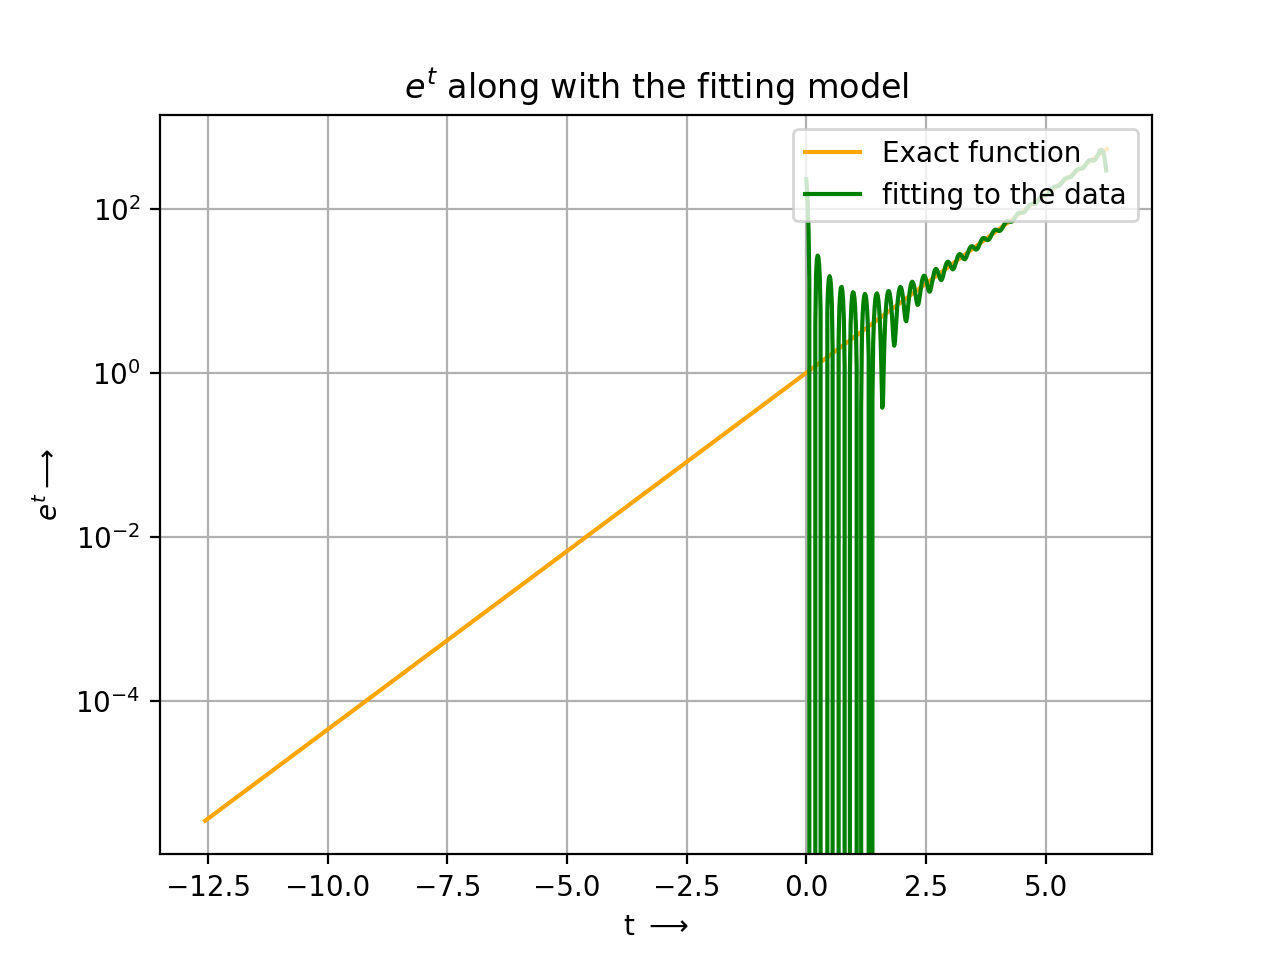
\includegraphics[scale=0.7]{Figure_1.png}}

\subsection{Plot of $cos(cos(t))$ along with the Estimated Function:}
% \begin{verbatim}
% figure(2)
% title('$cos(cos({t}))$'  ' along with the fitting model')
% plot(t,f_2(t),color='orange',label= 'Exact function')
% plot(x,matmul(A,p_coeff_2),color='green',label= 'fitting to the data')
% legend(loc="upper right")
% ylabel('$cos(cos({t}))$' '$\longrightarrow$')
% xlabel('t ' '$\longrightarrow$')
% \end{verbatim}
{\centering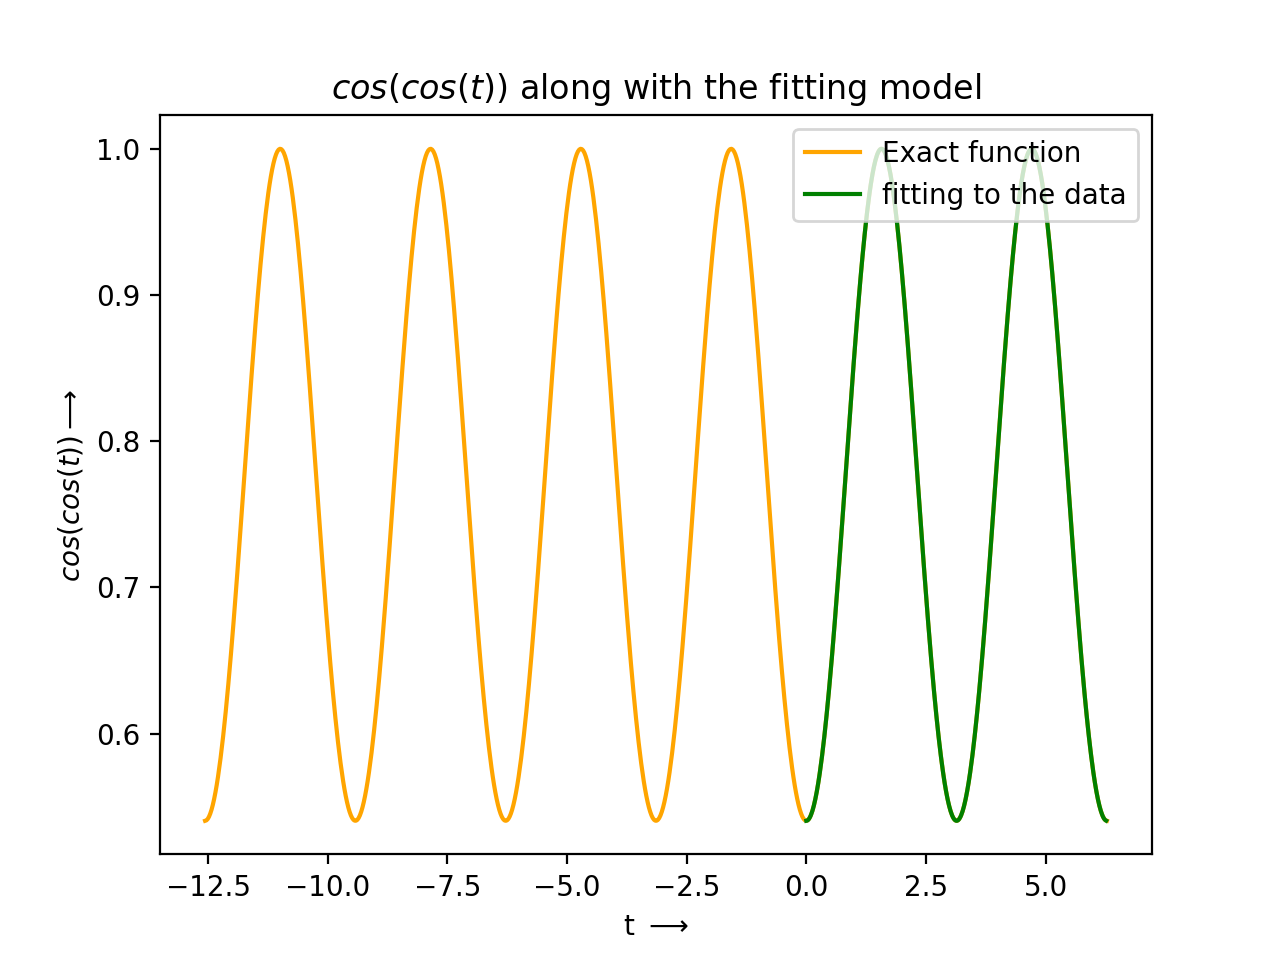
\includegraphics[scale=0.7]{Figure_2.png}}

\subsection{Plot of Coefficients of $e^t$ along with the Estimated Coefficients  in Semilog Scale:}
% \begin{verbatim}
% figure(3)
% title('coefficients of ' '$e^{t}$' ' by Fourier and Least Square method__semilogy')
% grid(True)
% semilogy(x_axis,coeff_1,color='orange',label= 'Fourier', marker='o', linestyle='')
% semilogy(x_axis,p_coeff_1,color='green',label= 'Lstsq', marker='o', linestyle='')
% legend(loc="upper right")
% ylabel('$e^{t}$' '$\longrightarrow$')
% xlabel('t ' '$\longrightarrow$')
% \end{verbatim}
{\centering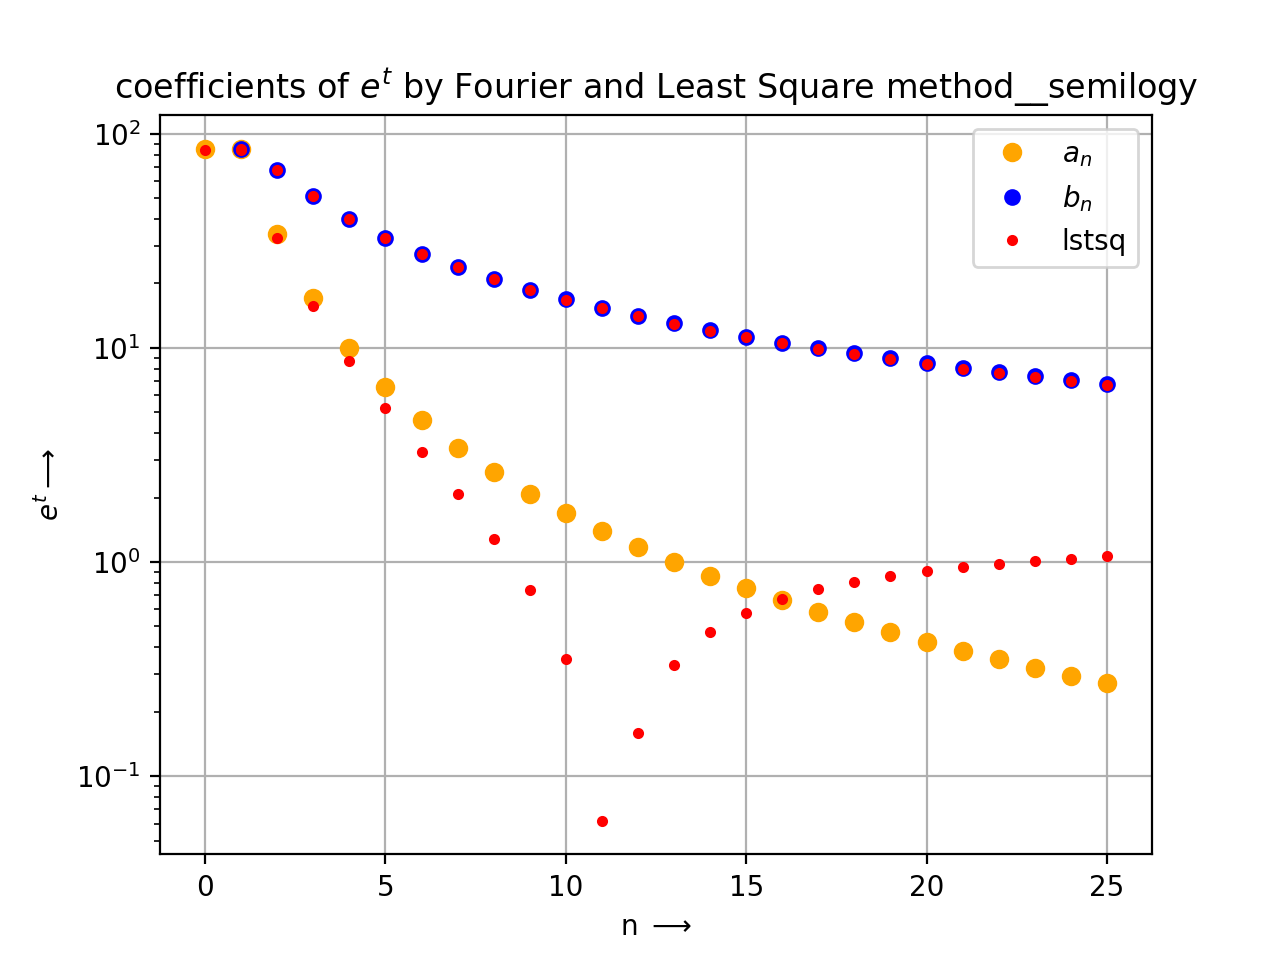
\includegraphics[scale=0.7]{Figure_3.png}}

\subsection{Plot of Coefficients of $e^t$ along with the Estimated Coefficients  in loglog Scale:}
% \begin{verbatim}
% figure(4)
% title('coefficients of ' '$e^{t}$' ' by Fourier and Least Square method__loglog')
% grid(True)
% loglog(x_axis,coeff_1,color='orange',label= 'Fourier', marker='o', linestyle='')
% loglog(x_axis,p_coeff_1,color='green',label= 'Lstsq', marker='o', linestyle='')
% legend(loc="upper right")
% ylabel('$e^{t}$' '$\longrightarrow$')
% xlabel('n ' '$\longrightarrow$')

% \end{verbatim}
{\centering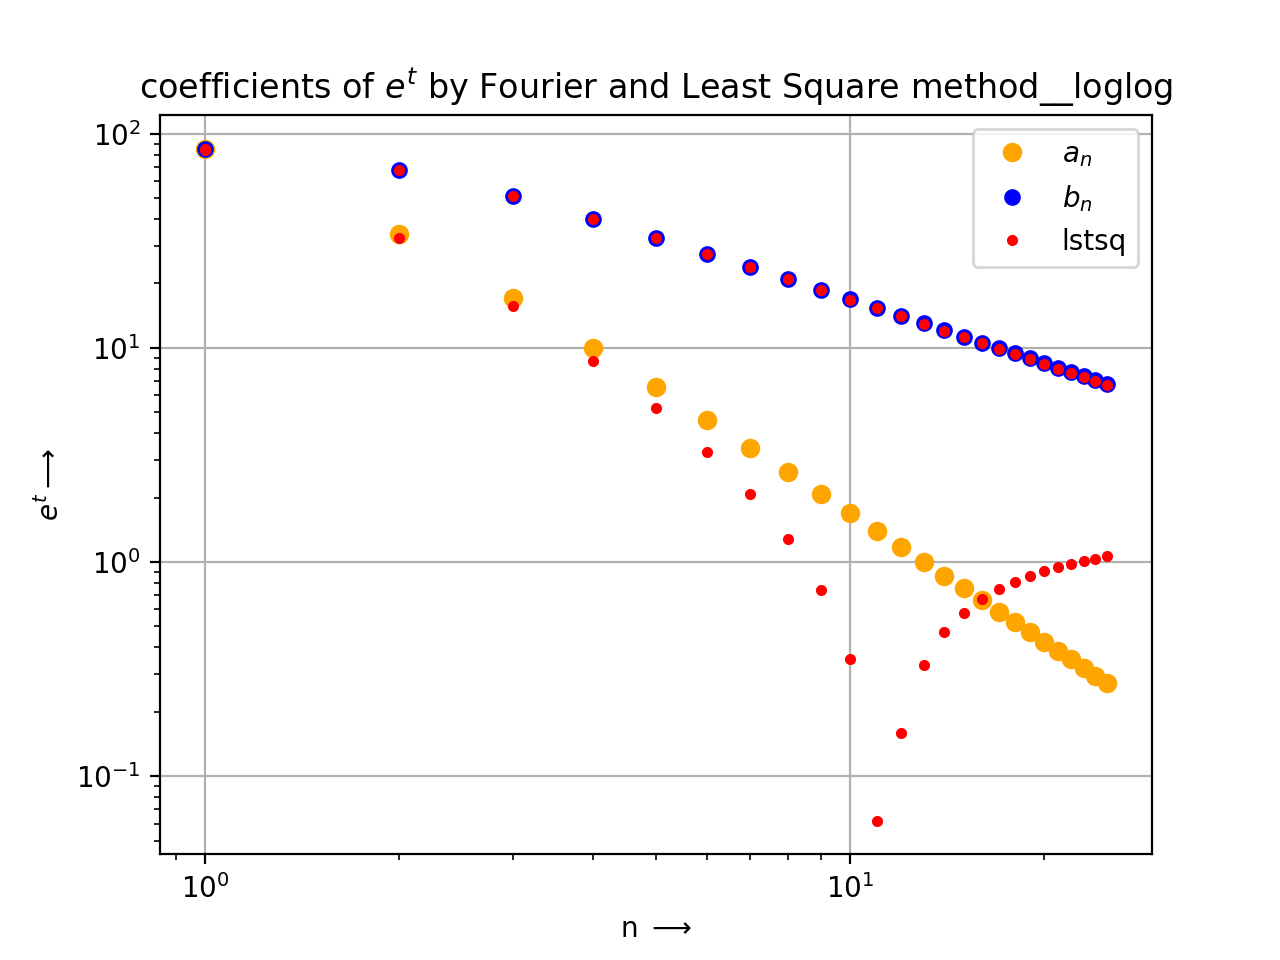
\includegraphics[scale=0.7]{Figure_4.png}}

\subsection{Plot of Coefficients of $cos(cos(t))$ along with the Estimated Coefficients  in Semilog Scale:}
% \begin{verbatim}
% figure(5)
% title('coefficients of ' '$cos(cos({t}))$' 'by Fourier and Least Square method__semilogy')
% grid(True)
% ylabel('$cos(cos({t}))$' '$\longrightarrow$')
% xlabel('t ' '$\longrightarrow$')
% semilogy(x_axis,coeff_2,color='orange',label= 'Fourier', marker='o', linestyle='')
% semilogy(x_axis,p_coeff_2,color='green',label= 'Lstsq', marker='o', linestyle='')
% legend(loc="upper right")
% \end{verbatim}
{\centering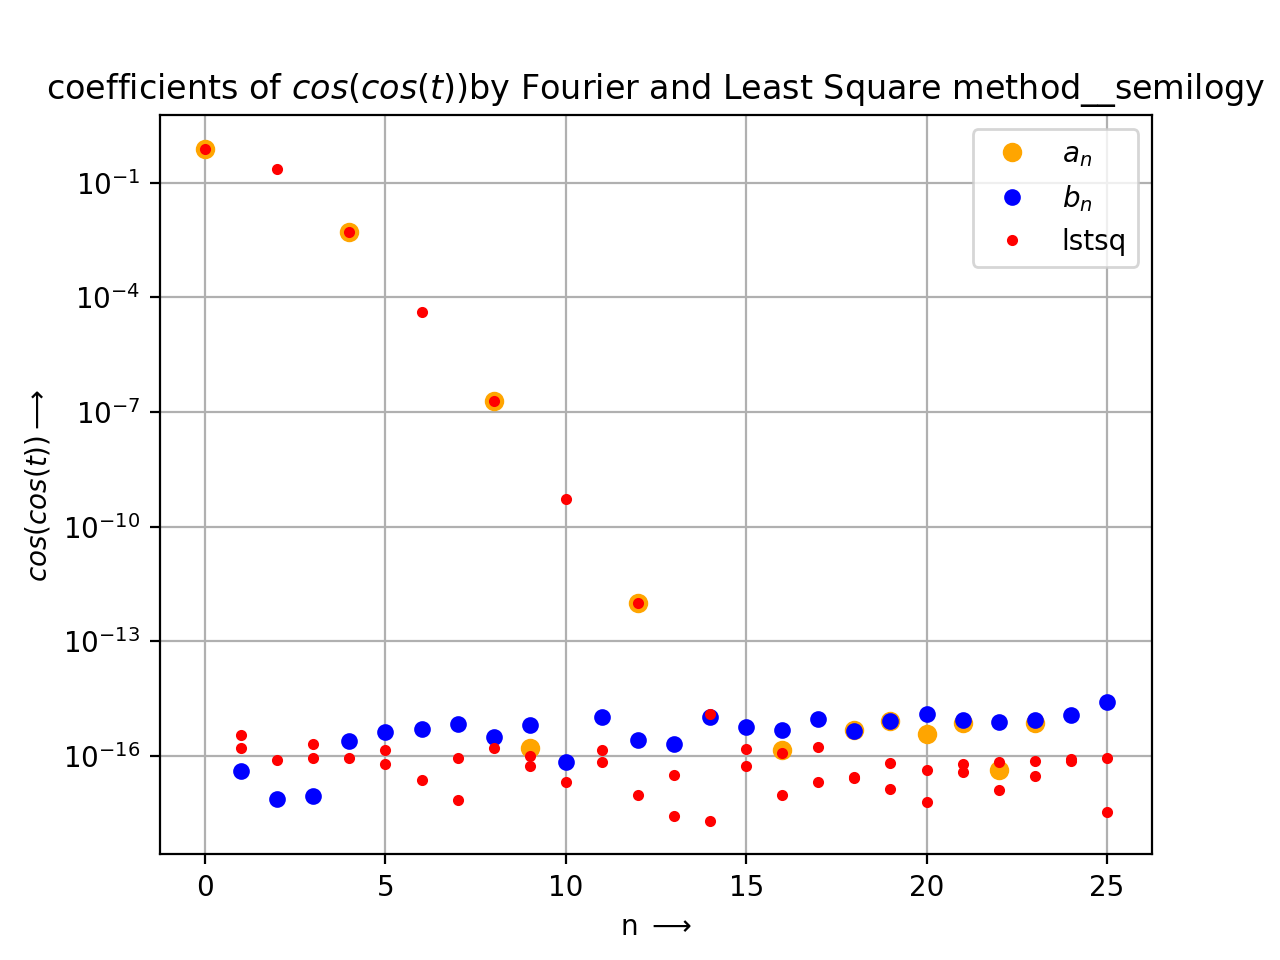
\includegraphics[scale=0.7]{Figure_5.png}}

\subsection{Plot of Coefficients of $cos(cos(t))$ along with the Estimated Coefficients  in Loglog Scale:}
% \begin{verbatim}
% figure(6)
% grid(True)
% title('coefficients of ' '$cos(cos({t}))$' 'by Fourier and Least Square method__loglog')
% loglog(x_axis,coeff_2,color='orange',label= 'Fourier', marker='o', linestyle='')
% loglog(x_axis,p_coeff_2,color='green',label= 'Lstsq', marker='o', linestyle='')
% legend(loc="upper right")
% ylabel('$cos(cos({t}))$' '$\longrightarrow$')
% xlabel('n ' '$\longrightarrow$')
% \end{verbatim}
{\centering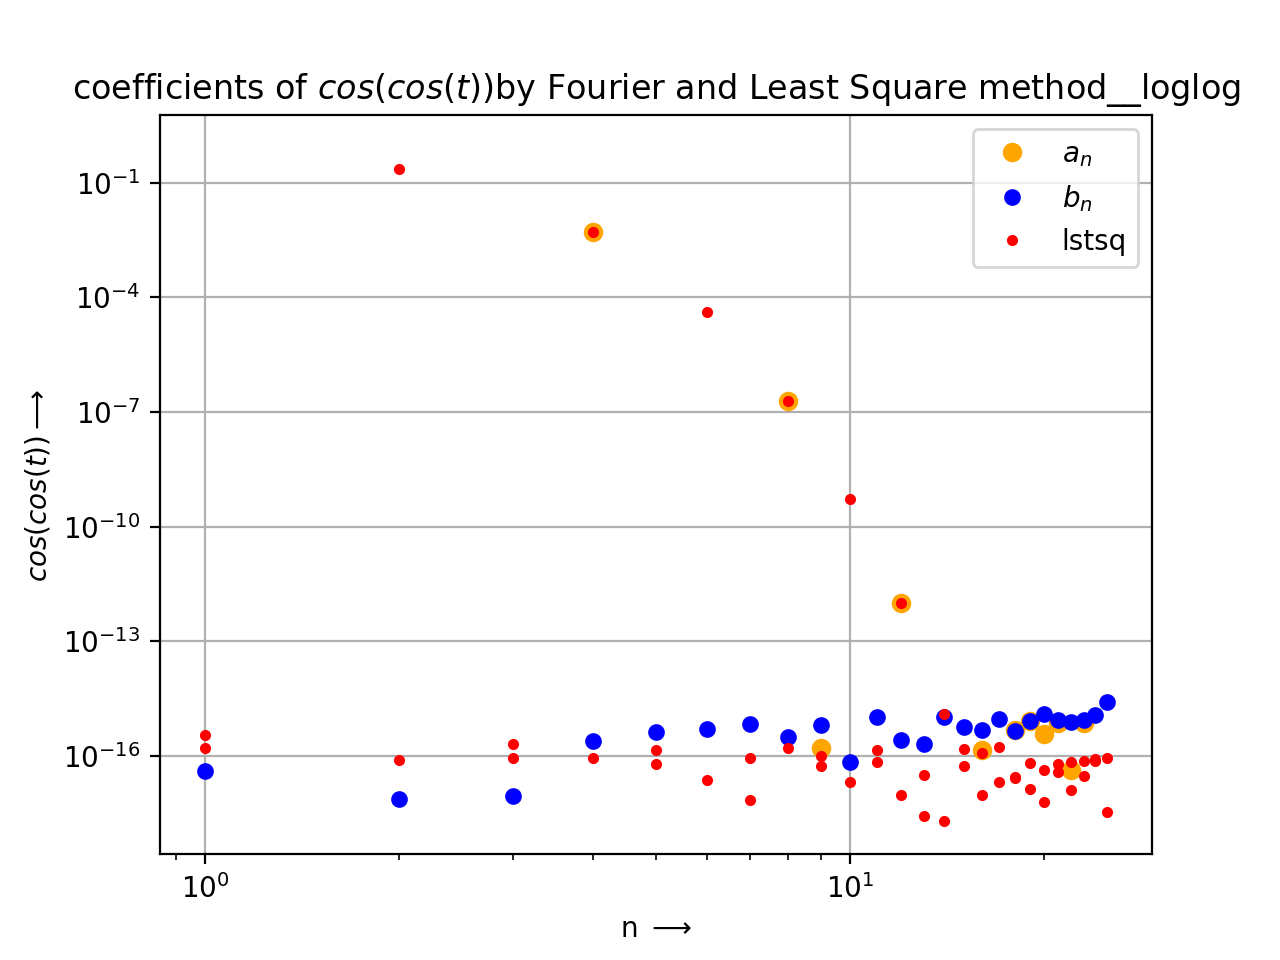
\includegraphics[scale=0.7]{Figure_6.png}}

\subsection{Deviation of Fourier coefficients from lstsq coefficients:}
% \begin{verbatim}
% figure(7)
% grid(True)
% title('Deviation of lstsq coeff. with fourier coeff.')
% plot(x_axis, abs(coeff_1-p_coeff_1), color='red', label=  'deviation for ' '$e^{t}$', marker='o', linestyle='')
% plot(x_axis, abs(coeff_2-p_coeff_2),color='blue', label= 'deviation for ' '$cos(cos({t}))$', marker='o', linestyle='')
% legend(loc="center right")
% ylabel('$(fourier\_coeff.) - (lstsq\_coeff.)$' '$\longrightarrow$')
% xlabel('n ' '$\longrightarrow$')
% \end{verbatim}
The below graph shows the absolute difference between the Fourier and lstsq coefficients.
{\centering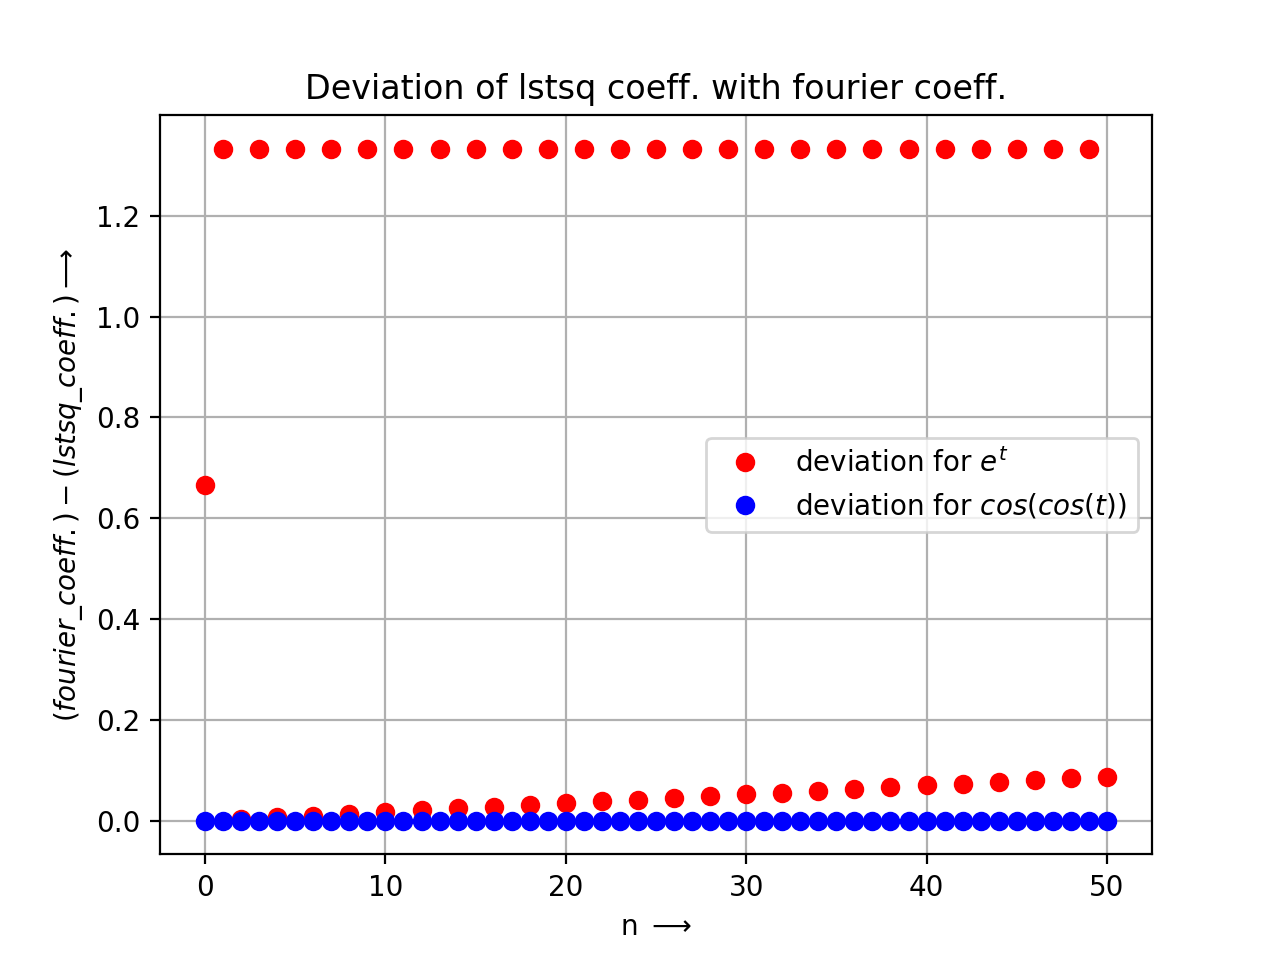
\includegraphics[scale=0.7]{Figure_7.png}}


\subsubsection{Finding the Maximun Deviation of the Coefficients:}
The max of the deviation of the lstsq coefficients with respect ot the Fourier coefficients can be computed as follows:\par

\begin{verbatim}
amax(abs(coeff_1-p_coeff_1))  ### by using amax function
amax(abs(coeff_2-p_coeff_2))
\end{verbatim}

The $amax$ function returns the maximun value in the input array. And the output is shown below:\par
{\centering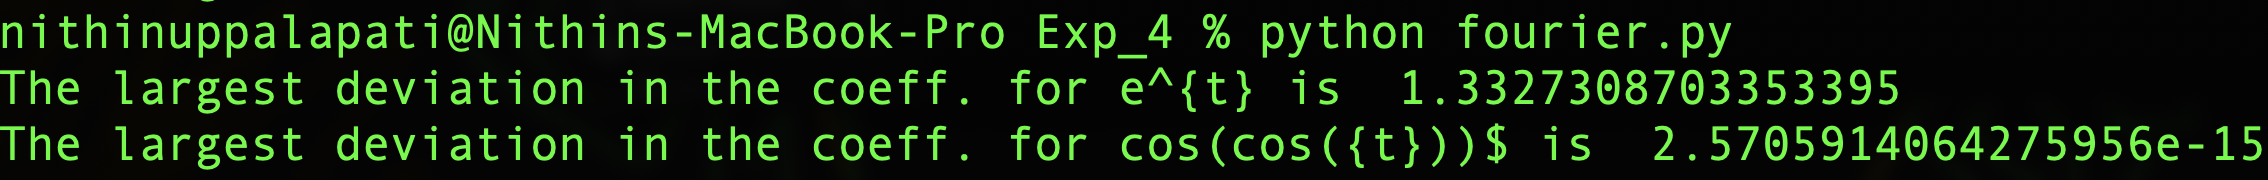
\includegraphics[scale=0.44]{output.png}}


\chapter{Conclusions}
\section{On the Deviation of Coefficients:}
So,  as $cos(cost)$ is periodic with period $\pi$, and which is equal to the twice of the fundamental period $2\pi$, 

\begin{verbatim}
amax(abs(coeff_1-p_coeff_1))  ### by using amax function
amax(abs(coeff_2-p_coeff_2))
\end{verbatim}
\subsection{Comment on Lstsq, and Fourier Coefficients:}
\begin{itemize}
\item So, as we are computing the first few Fourier coefficients, whereas in lstsq method, we are trying to fit the entire function to the $51$ coefficients, the two sets of coefficients are not going to be the same.
\end{itemize}

\begin{itemize}
\item So, in order to account the entire function, the first few coefficients will deviate and gradually they are in good agreement.
\end{itemize}

\begin{itemize}
\item And in the case of Fourier coefficients of $cos(cost)$, the $b_n's$ are nearly zero, (\textit{actually they should be exactly zero, but it is not; due to the floating error while computing...}) as the function, $cos(cost)$ is an even function.
\end{itemize}

\begin{itemize}
\item And in the case of Fourier coefficients of $e^t$, they are not decaying as in the case of $cos(cost)$, because, the function $e^t$ is not a periodic function, and thus it contains all harmonics of the fundamental frequency.
\end{itemize}


% \pagebreak


% \pagebreak

\end{document}

